
\subsection{Academic Direction and Oversight}

\bsaicommittee{The academic director of the program will be tenured faculty in computer
science with a dual report to both \aim{}'s Associate Director of
Education and the Chair of the \abr{cs} department.}

\csamend{The program will be under the direction of the Department of Computer Science and AIM. A tenured faculty in the Department of Computer Science holding a joint appointment with AIM will serve as the BS in AI Academic Director. The Academic Director will be appointed by the Chair of the Department of Computer Science with approval of the CMNS Dean and the AIM Director, and report to the Chair of the Department of Computer Science and to AIM's Associate Director of Education. The Academic Director will coordinate with AIM to align the program with AIM’s strategic objectives in close collaboration with AIM staff.}

\csamend{The Academic Director will provide overall leadership and operational oversight of the program, and supervise the program staff including the Assistant Program Director and the Academic Advising team led by an Assistant Director.}

Adopting, proposing, and amending the program will fall under the purview of the PCC (Program, Courses, and Curricula) and VPAC (Vice President's Advisory Committee) processes of the Computer Science department and its Education Committee after approval of the \short{} committee.  
%This committee will have representatives from Math, INFO, and ARHU in addition to two members from Computer Science (each nominated by their home units) in addition to at most two members nominated by the director of \aim{}.  
The proposal and amendment of individual courses will be the purview of the unit(s) responsible for offering the course.

The members of the committee developing the proposal are:
\begin{itemize}
    \item Eric Pacuit (Phil)
    \item Roger Eastman (CS)
    \item Pratap Tokekar (CS)
    \item Vanessa Fr\'ias-Martinez (Info)
    \item Lizhen Lin (Math)
    \item Jordan Boyd-Graber (chair, CS)
    \item Xianfeng Yang (ECE)
\end{itemize}

Their titles, credentials, and potential courses are in an
attachment.  Alyssa Ryan (the Director of Academic Programs for
\abr{aim}) is coordinating the development of the program in the
broader landscape of the \abr{aim} initiative.

\subsection{Administrative Coordination}

%\begin{figure}
 % \begin{center}
%    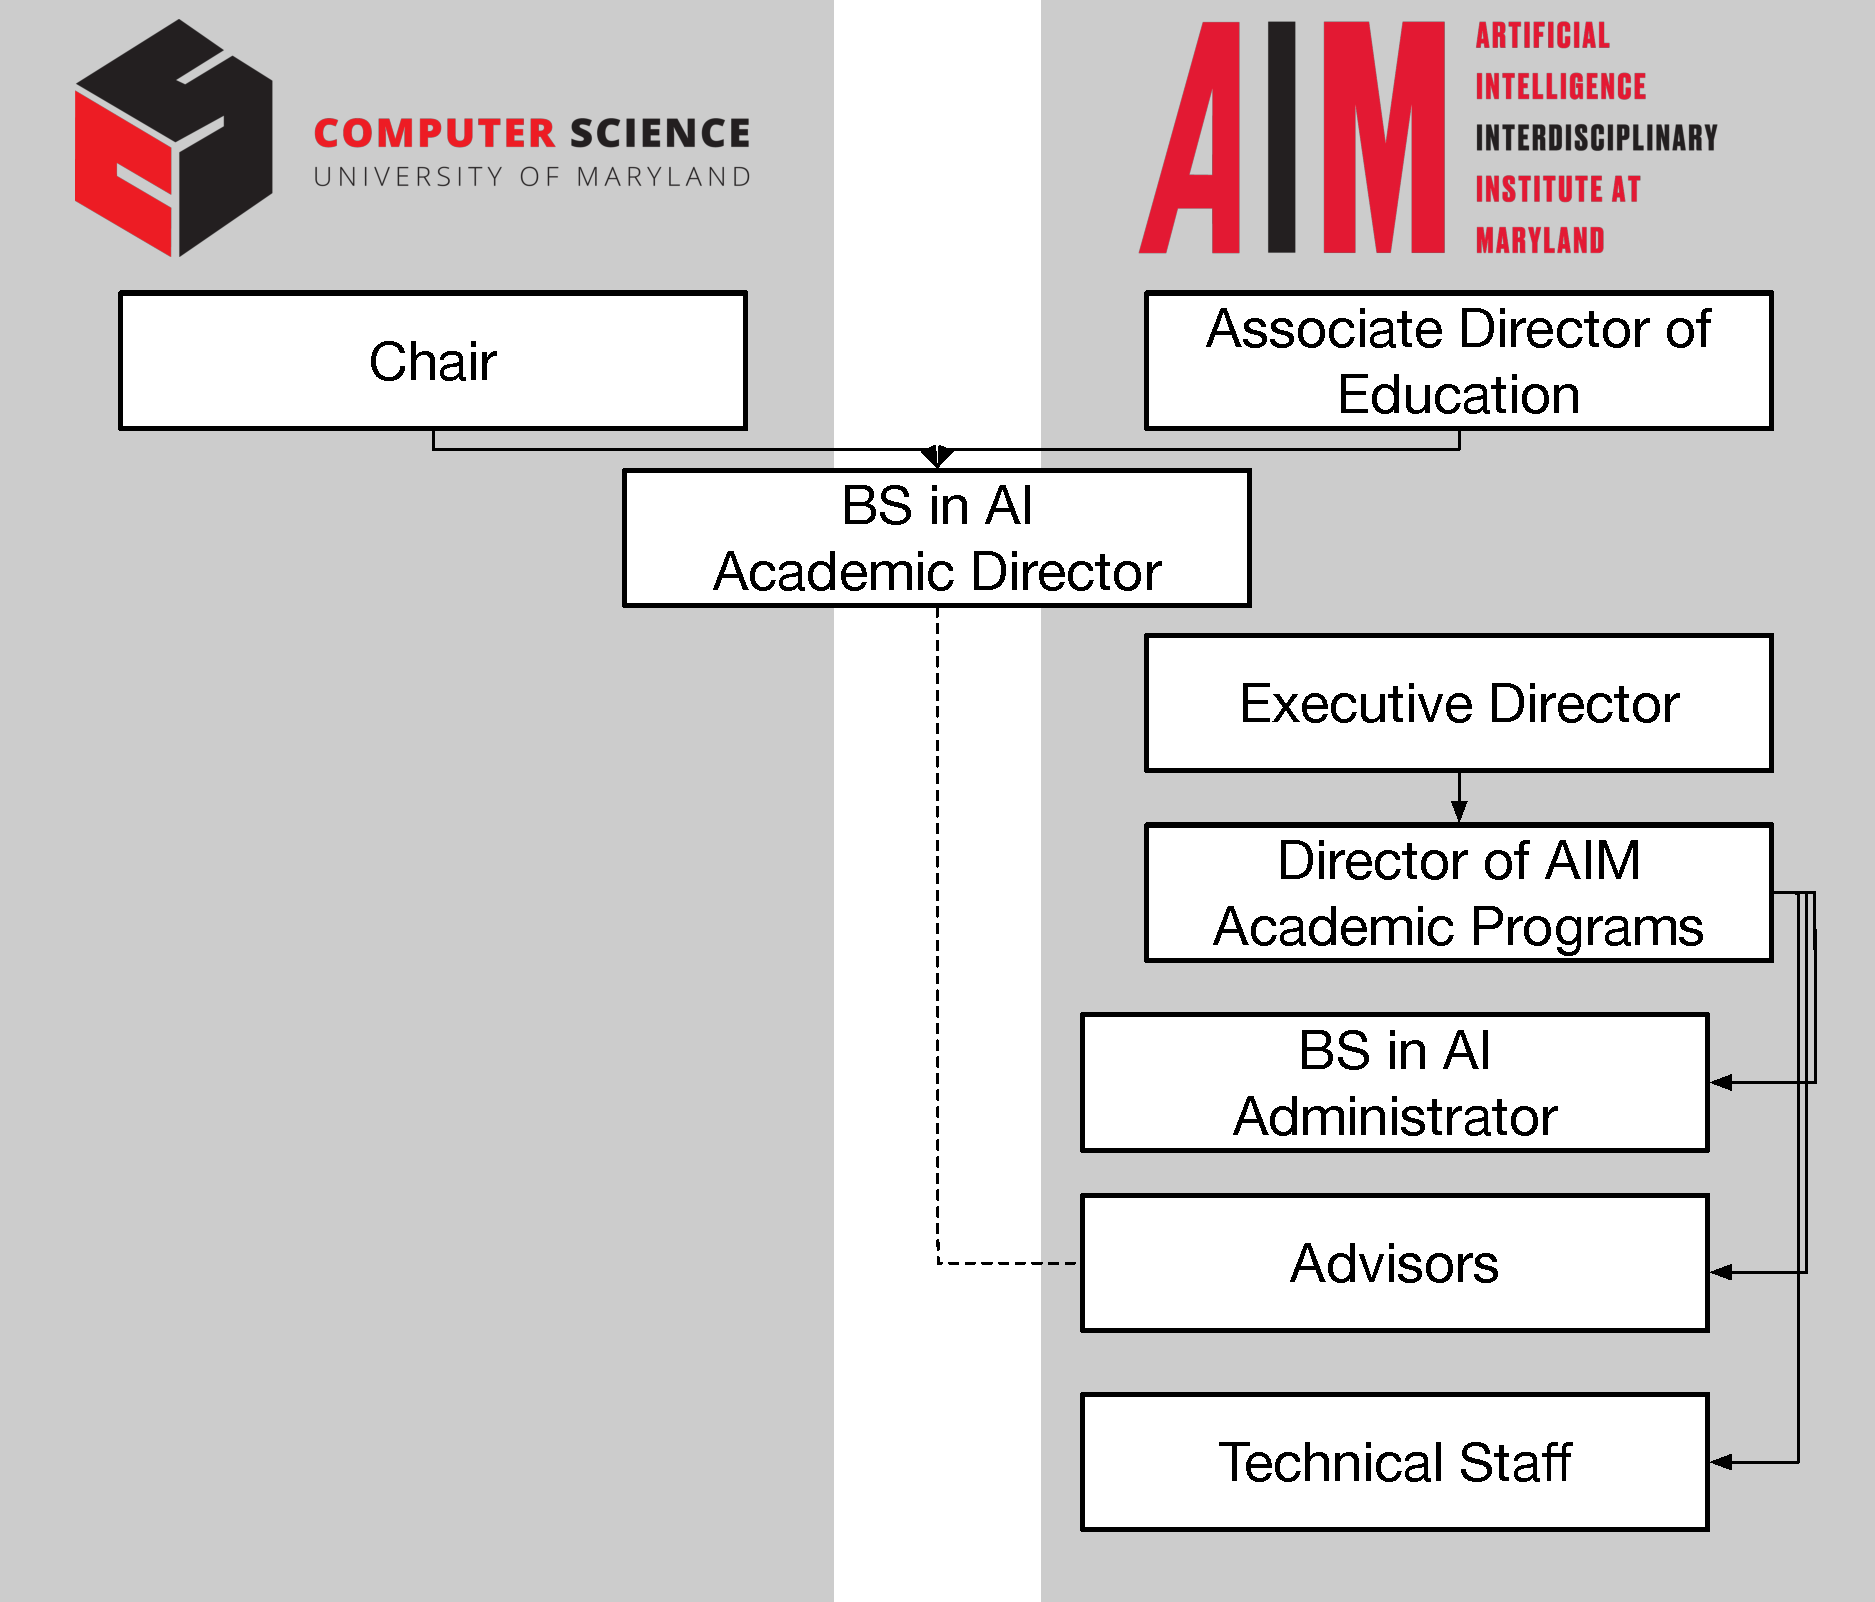
\includegraphics[width=0.5\linewidth]{figures/aim_org_chart}
%  \end{center}
%  \caption{\bsaicommittee{Organization chart for \short{}.}}
%  \label{fig:org_chart}
%\end{figure}

\begin{figure}
  \begin{center}
    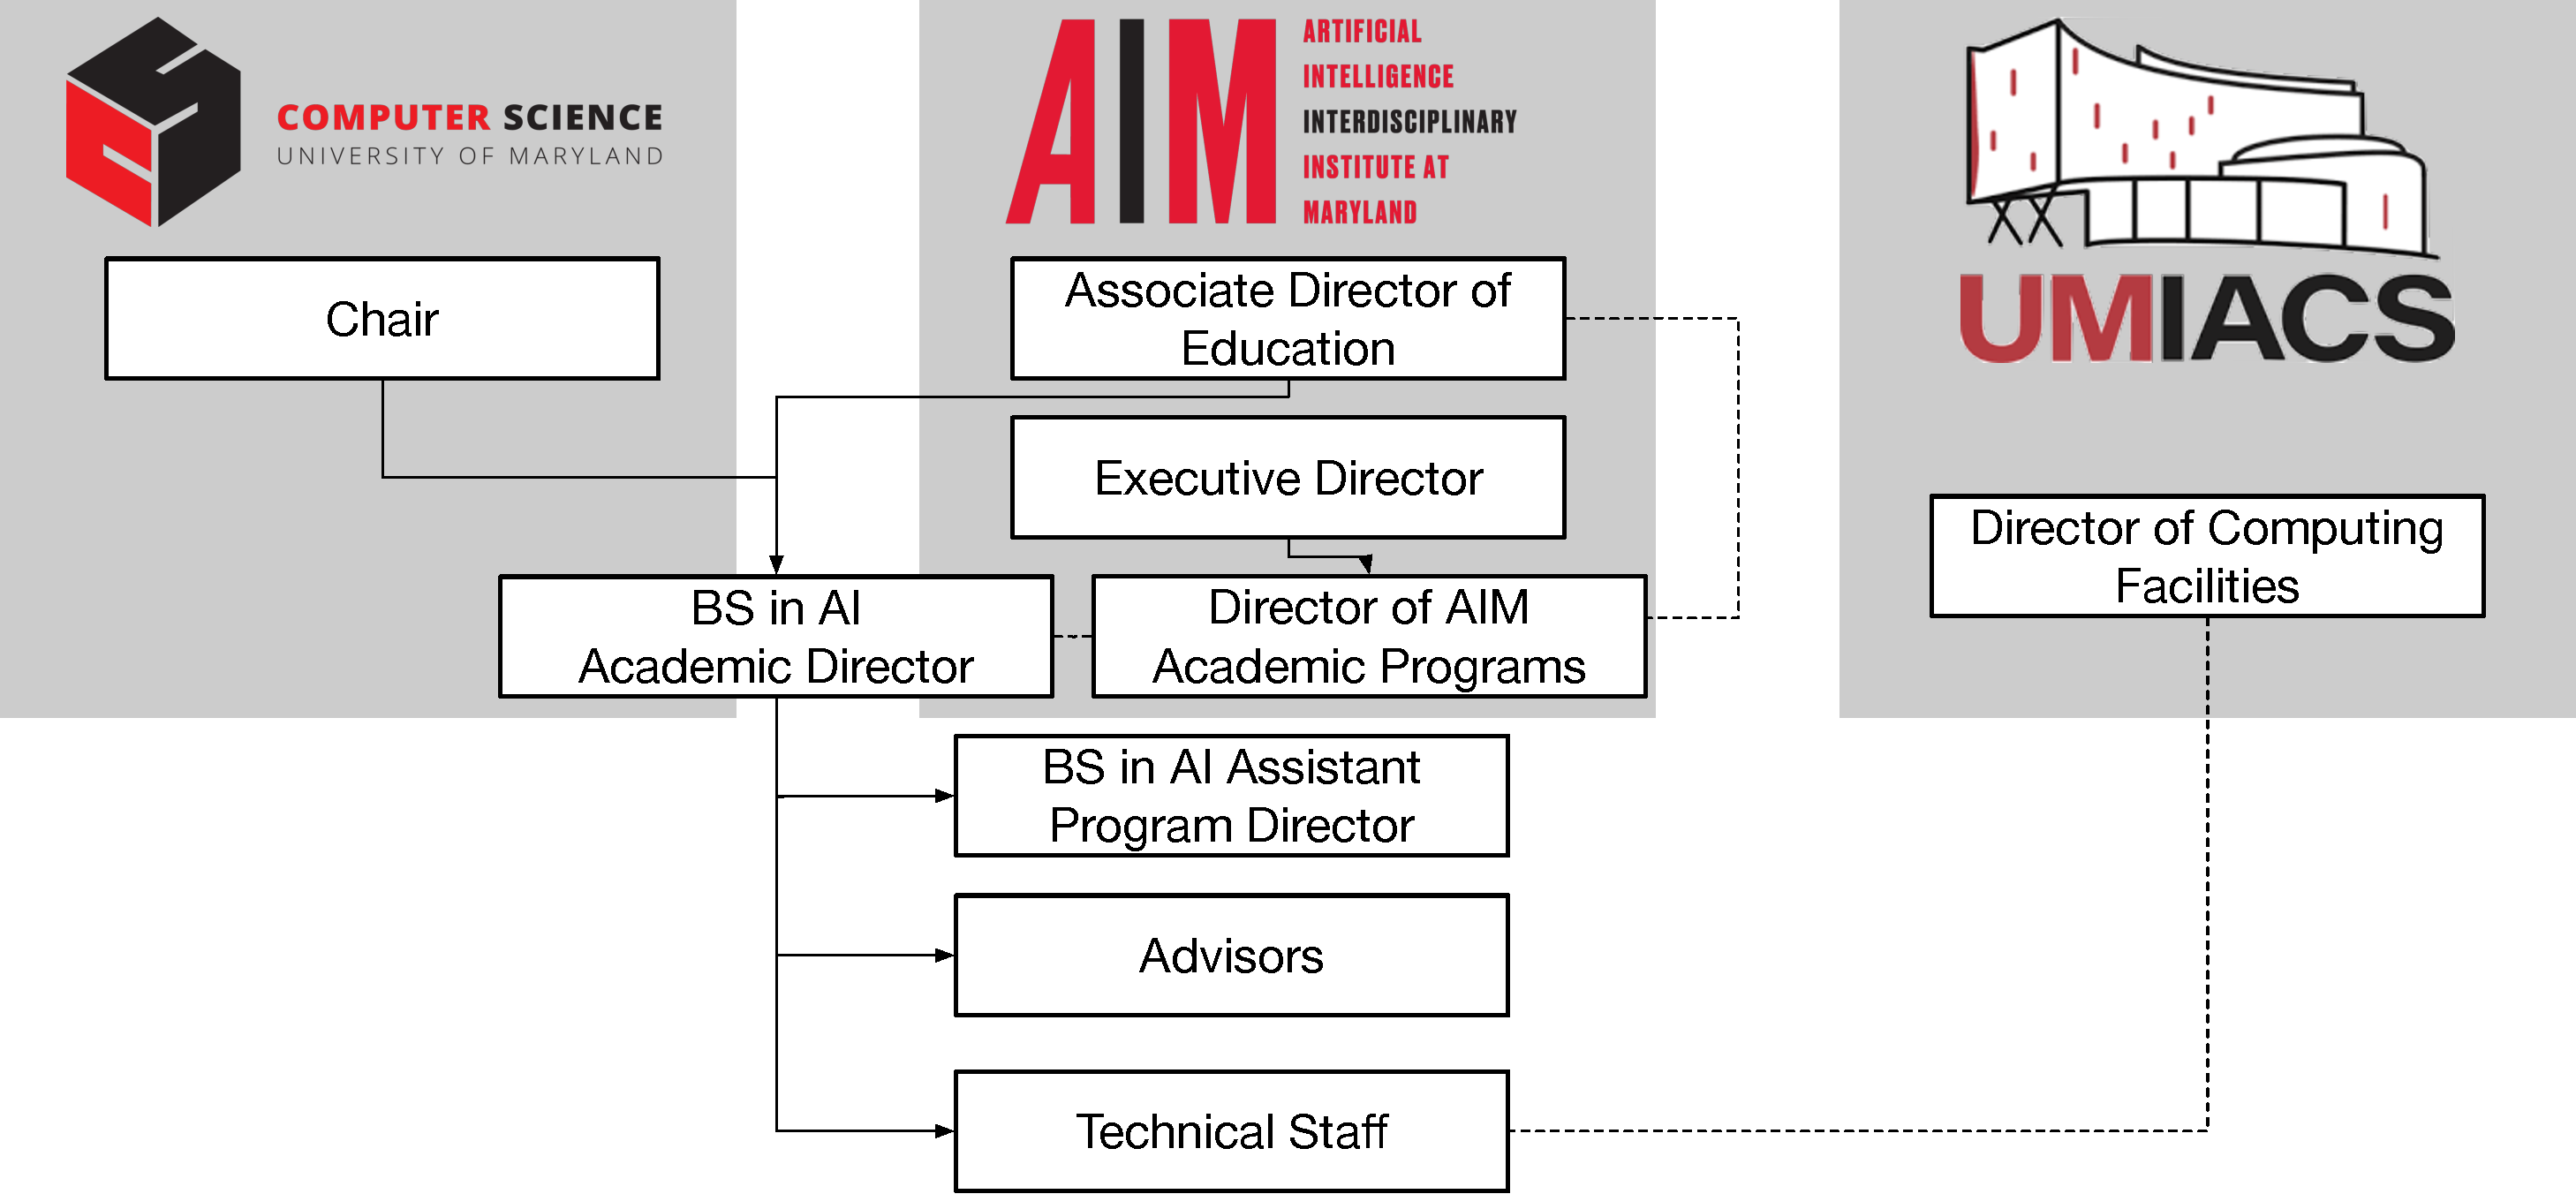
\includegraphics[width=0.75\linewidth]{figures/cs_org_chart}
  \end{center}
  \caption{\csamend{Organization chart for \short{}.}}
  \label{fig:org_chart}
\end{figure}


\bsaicommittee{The program will be administered jointly by computer science and \aim{}. There will be a staff Program Administrator who will report to the Program Director, and closely coordinate with the \aim{} Associate Director of Education.}

\csamend{A full-time Assistant Program Director for the proposed major will be responsible for administrative leadership of the program. In addition, there will be an academic advising team led by an Assistant Director. Finally, a technical staff member will coordinate technical resources including high performance computing. The Assistant Program Director and the Assistant Director for academic advising will be supervised by the Academic Director of the BS in AI. The technical staff will be supervised by appropriate AIM staff and coordinate with appropriate technical leadership of the Nexus cluster (currently part of \abr{umiacs}).}

